\section{CADO: Computer Aided Design Optimization Tool}
\todourgent[inline,author=Benni]{How did we put together the different parts? Here mainly first part of presentation: workflow, overview, user experience}
\begin{figure}
\begin{subfigure}[t]{.49\textwidth}
\centering
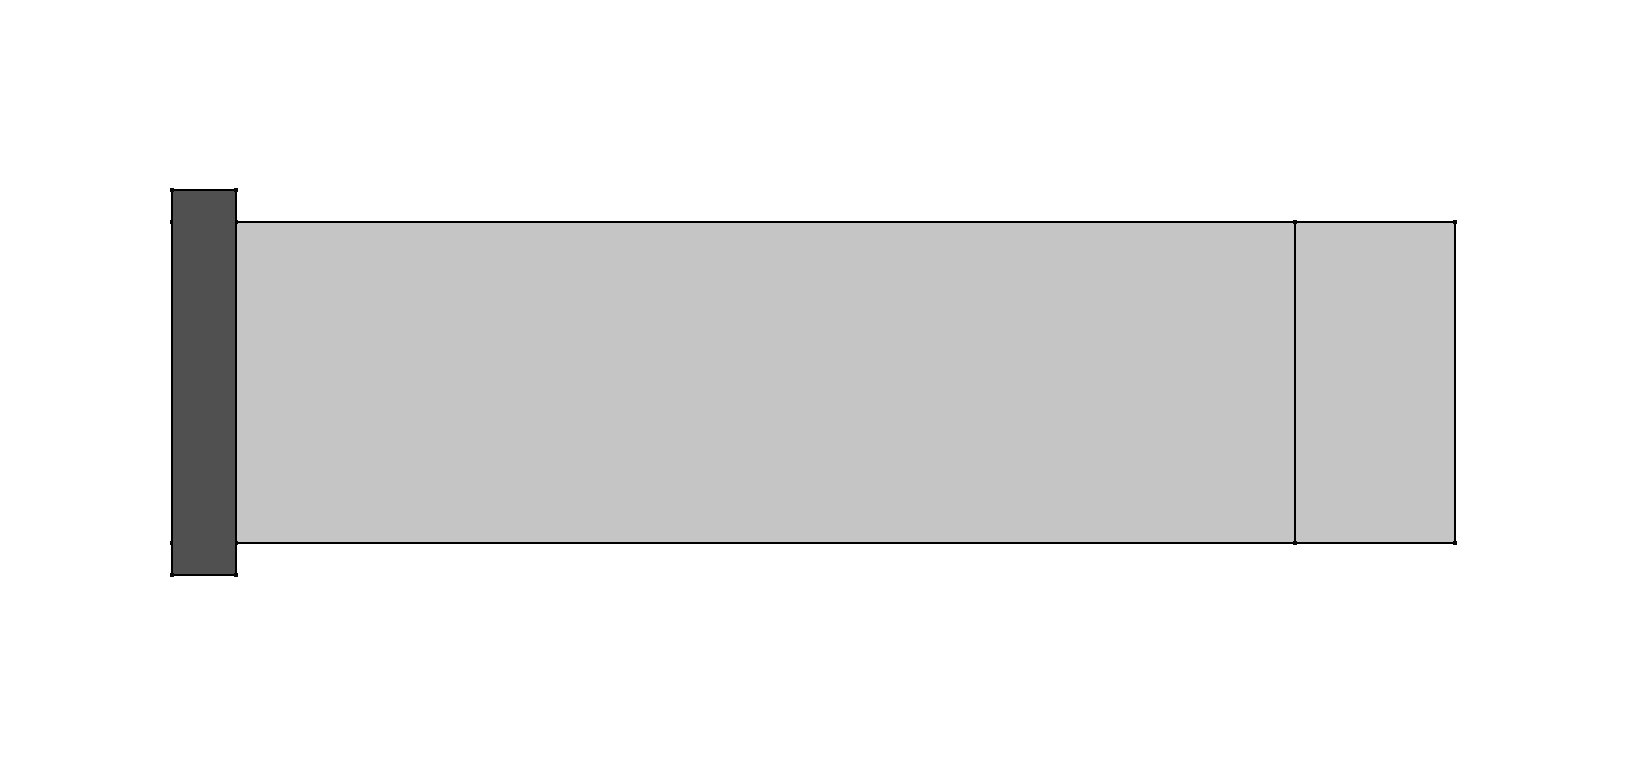
\includegraphics[width=\textwidth]{Pictures/CADO_Overview/Back2CAD1.png}
\caption{Initial geometry file}
\end{subfigure}
\begin{subfigure}[t]{.49\textwidth}
\centering
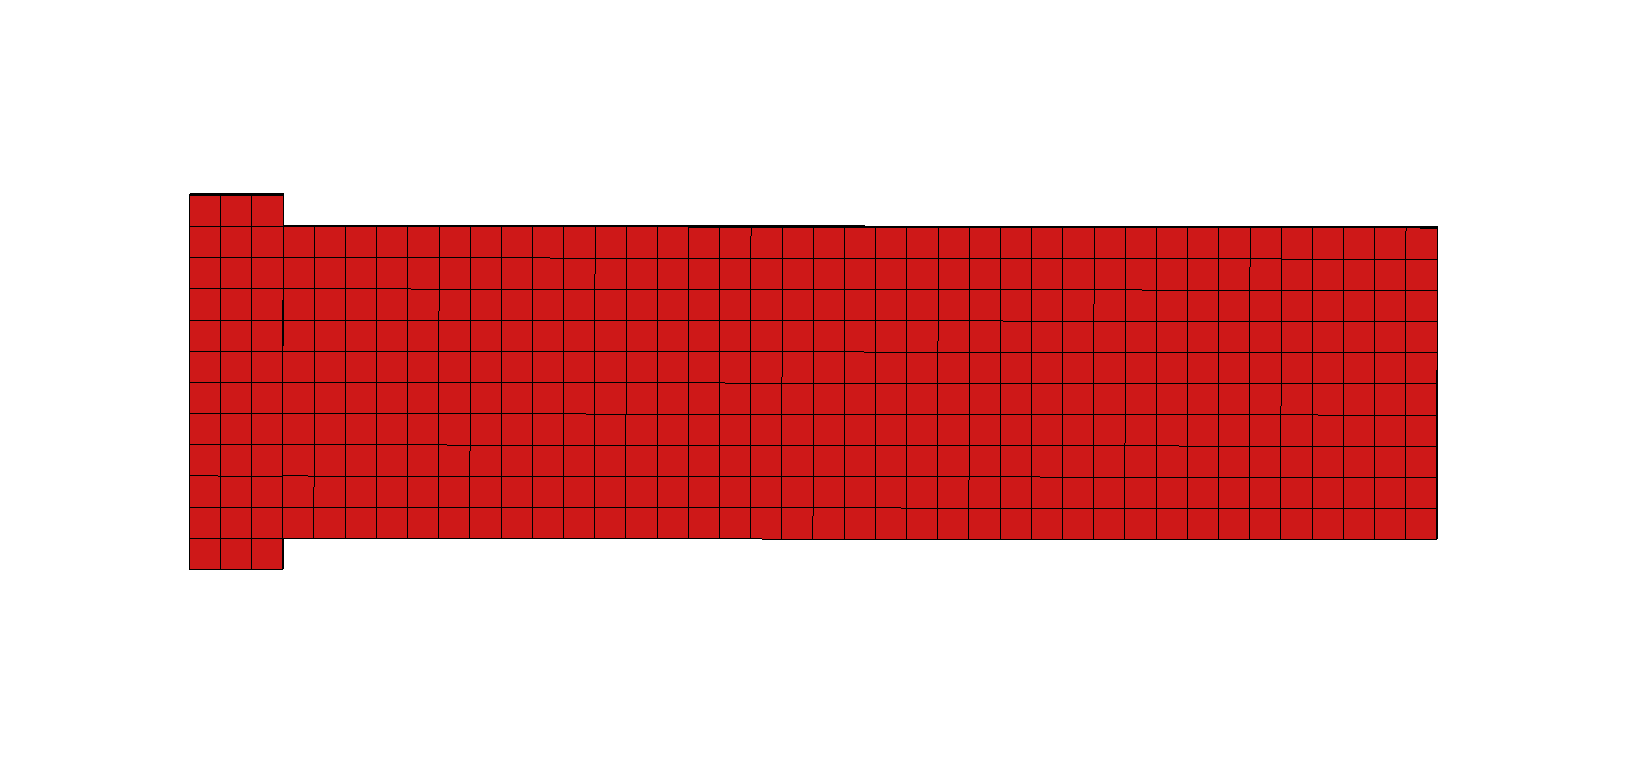
\includegraphics[width=\textwidth]{Pictures/CADO_Overview/Back2CAD2.png}
\caption{Voxelized input geometry}
\end{subfigure}
\begin{subfigure}[t]{.49\textwidth}
\centering
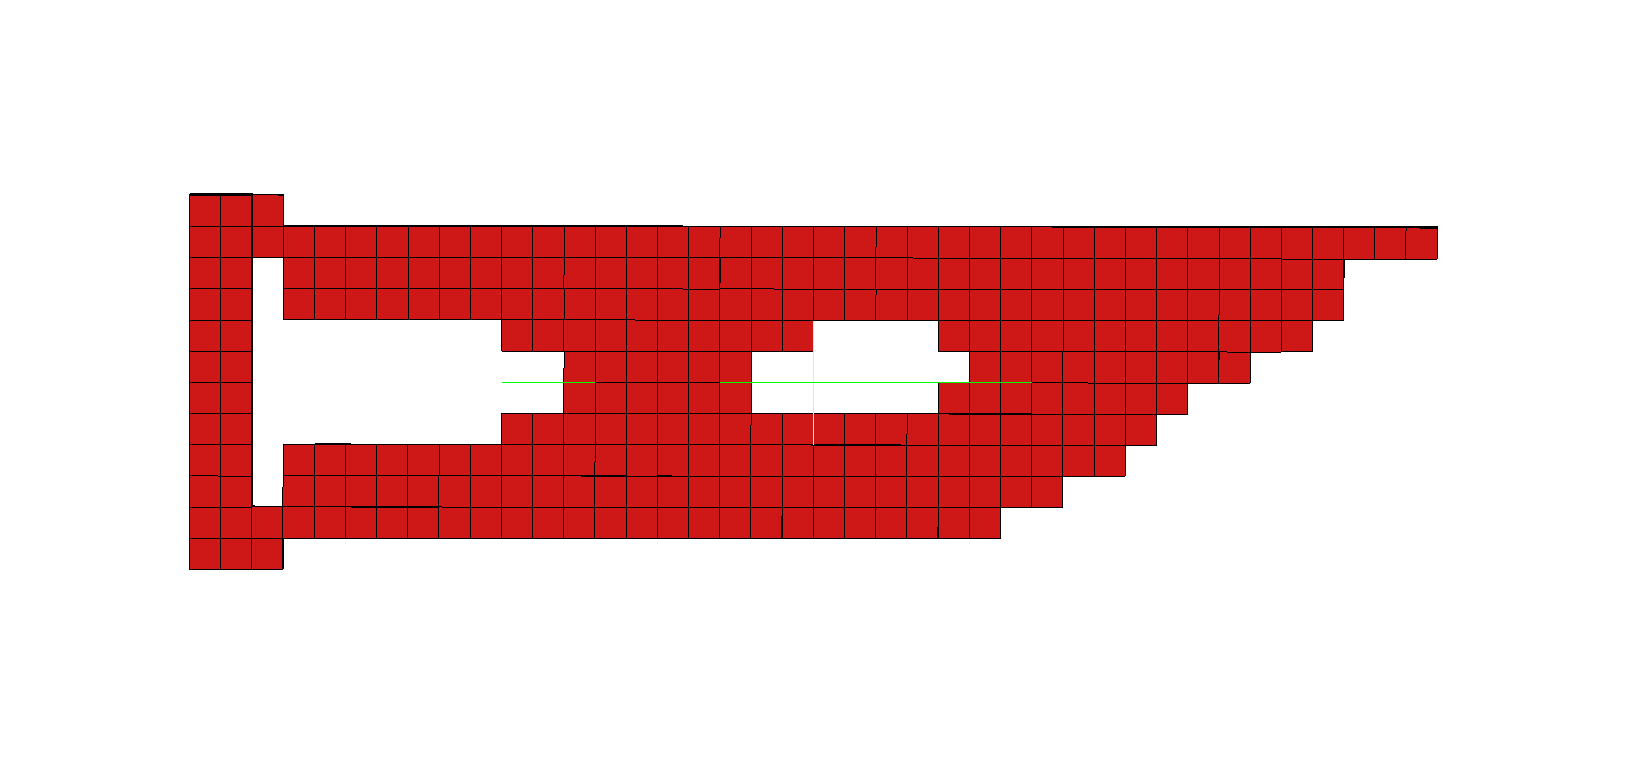
\includegraphics[width=\textwidth]{Pictures/CADO_Overview/Back2CAD3.png}
\caption{Optimized voxel raster}
\end{subfigure}
\begin{subfigure}[t]{.49\textwidth}
\centering
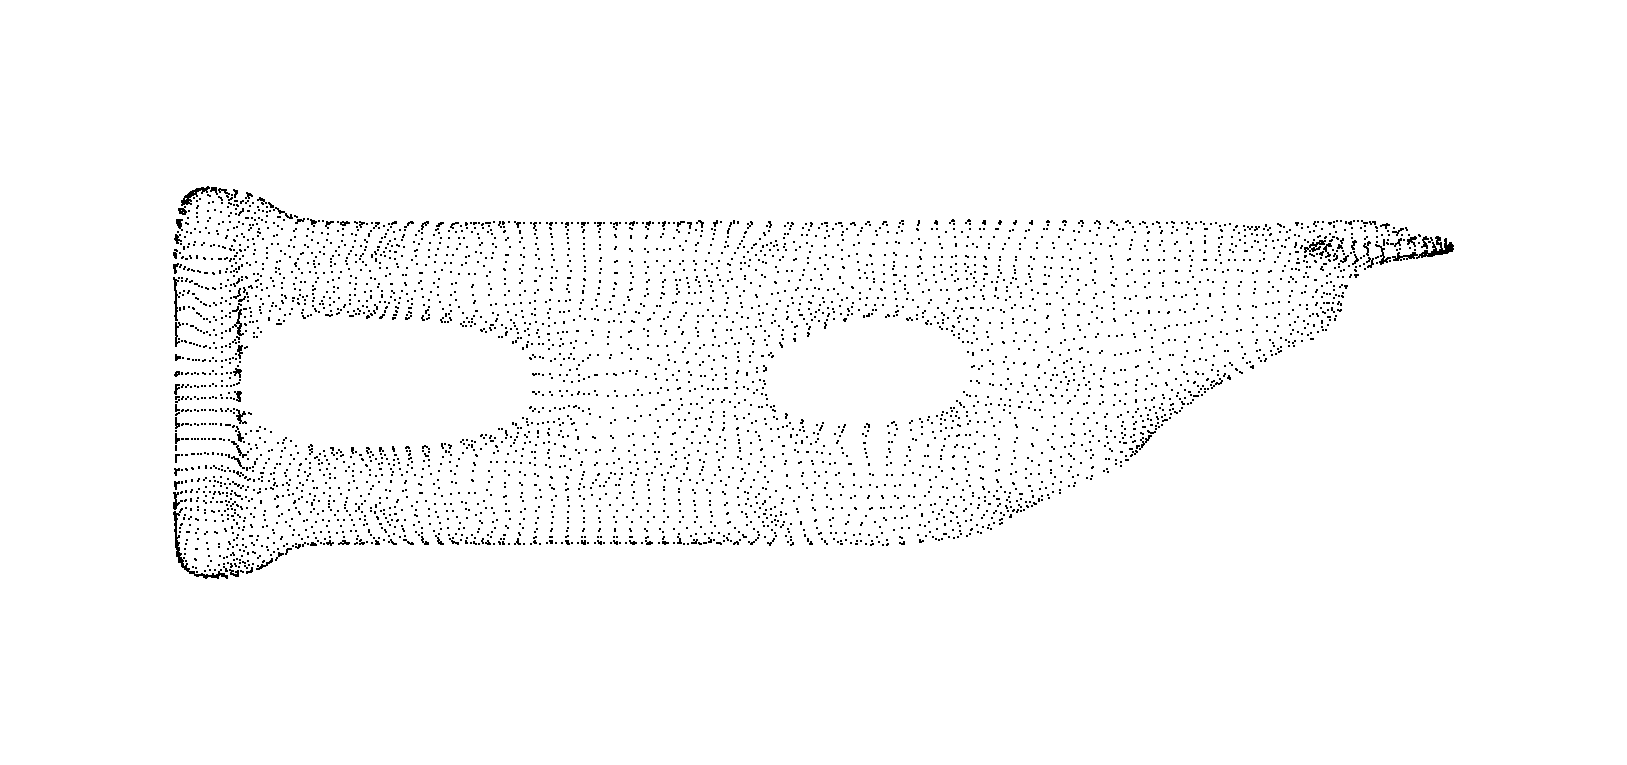
\includegraphics[width=\textwidth]{Pictures/CADO_Overview/Back2CAD4.png}
\caption{Point cloud obtained by Dual Contouring}
\end{subfigure}
\begin{subfigure}[t]{.49\textwidth}
\centering
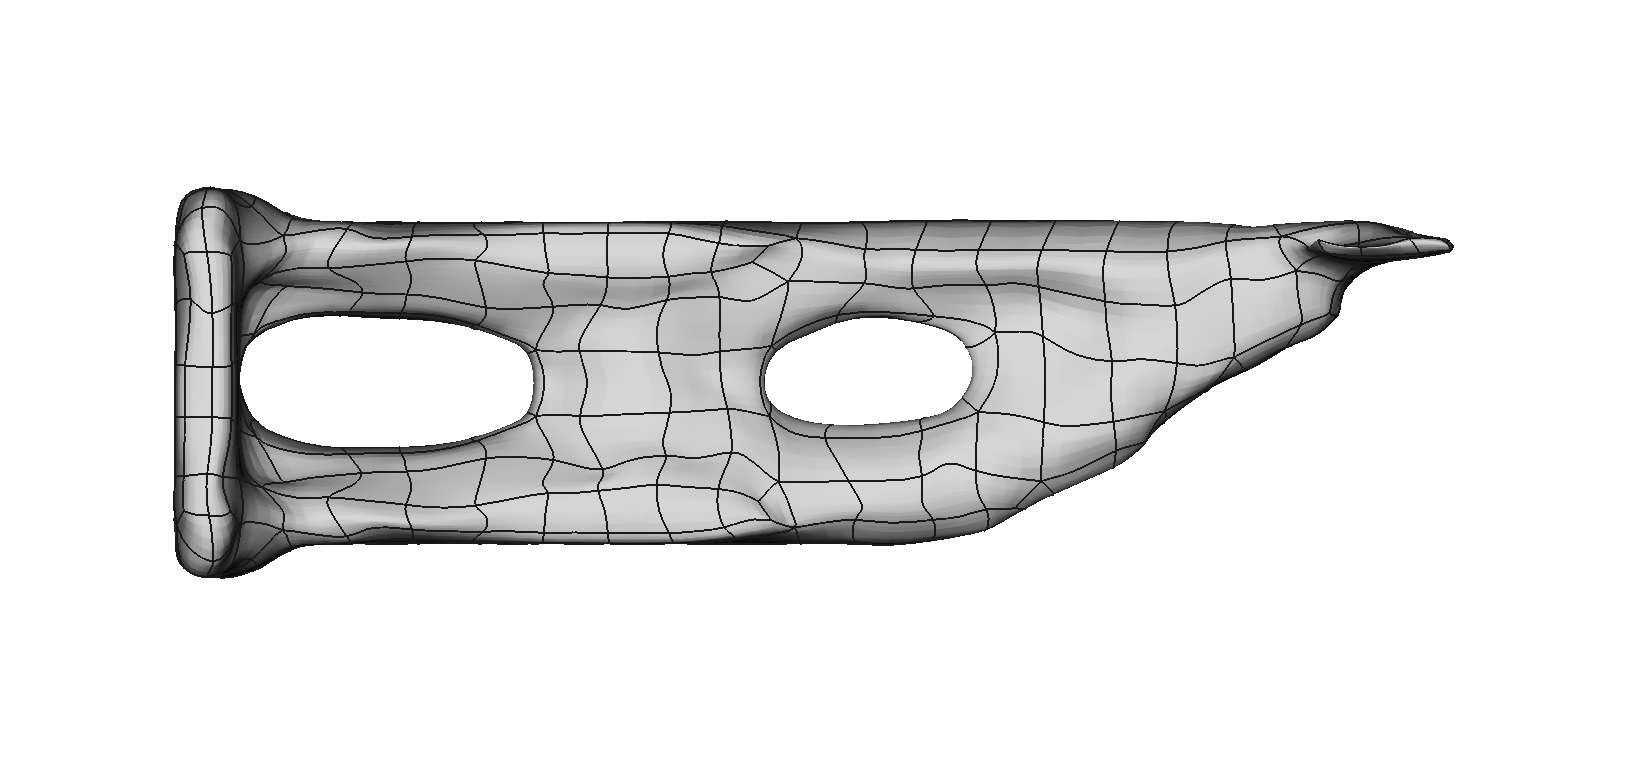
\includegraphics[width=\textwidth]{Pictures/CADO_Overview/Back2CAD5.png}
\caption{B-Spline surface}
\end{subfigure}
\begin{subfigure}[t]{.49\textwidth}
\centering
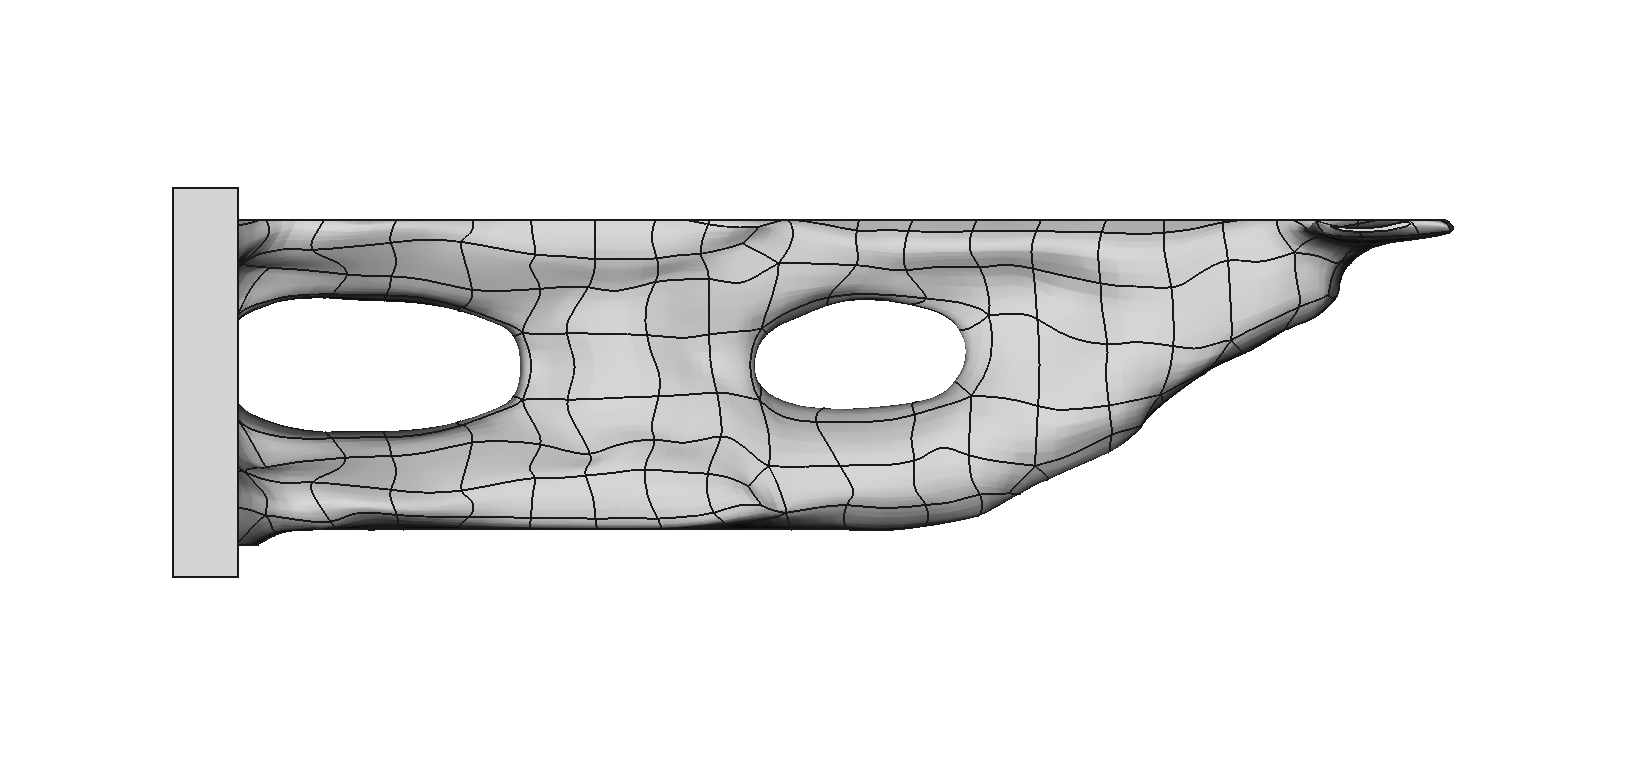
\includegraphics[width=\textwidth]{Pictures/CADO_Overview/Back2CAD6.png}
\caption{Boolean fusion with non-changing domain}
\end{subfigure}
\caption{Overview of workflow stages imposed by CADO}
\end{figure}

\todointernal[inline,author=Benni]{Add more pictures in that style for the remaining parts?}